% -- Proyecto Ars_Mathematica
% https://www.instagram.com/ars_mathematica/
%
% Autor:		Rodrigo Sánchez-Martínez
% Fecha:		17 de abril del 2024
% Contacto:		rodrigo.smtz@icloud.com
%
% Descripción de la figura:
% 	Ecuaciones polares de la elipse desde dos perspectivas:
%	1. con el centro en el origen
%	2. con uno de sus focos en el orgen
%
% Licencia:
%	Este código puede ser distribuido libremente. El objetivo de este proyecto es compartir con ustedes un poco de las herramientas que utilizo en TikZ y que he aprendido con la experiencia. Por favor, no duden en contactarme si tienen alguna duda o si hay algun error tanto en la parte del código de LaTeX, como en la descripción matemática y física de los conceptos.
%
%	Rodrigo.

\documentclass[border = 1mm, tikz]{standalone}

% -- Paqueterías importantes

% entrada
\usepackage[utf8]{inputenc}
% matemáticas
\usepackage{amsmath}

% TikZ
\usepackage{tikz}
\usetikzlibrary{
	scopes, backgrounds,
	angles, quotes,
	math
}

% Tamaño del dibjo completo
\def\L{8} % cm

% -- Cuerpo del documento
\begin{document}

% Página 1
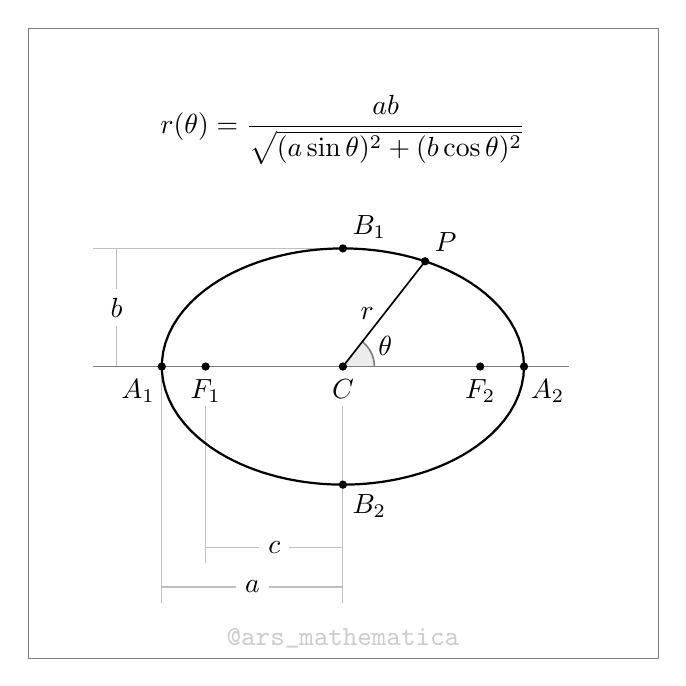
\begin{tikzpicture}

	% márgenes del dibujo
	\draw[help lines] (0,0) rectangle (\L,\L);

	% desplazamiento del origen de coordenadas al centro de la imagen
	\begin{scope}[shift = {(0.5*\L,0.5*\L - 0.3)}]
		
		% definición de las variables
		\tikzmath{
			% parámetros de la elipse
			\a = 2.3; \b = 1.5;
			\c = sqrt((\a)^2 - (\b)^2);
			% ec. de la elipse 
			function f(\x) {
				return \a*\b/sqrt((\a*sin(\x))^2 + (\b*cos(\x))^2);
			};
		};
		
		% expresión
		\node at (0,3) {
			$r(\theta) =
			\dfrac{ab}{\sqrt{(a\sin\theta)^2 + (b\cos\theta)^2}}$
		};
		
		% def. de las coordenadas importantes
		\coordinate (C) at (0,0);
		\coordinate (F1) at (-\c,0);
		\coordinate (F2) at (+\c,0);
		\coordinate (A1) at (-\a,0);
		\coordinate (A2) at (+\a,0);
		\coordinate (B1) at (0,+\b);
		\coordinate (B2) at (0,-\b);
		
		% elección de un punto arbitrario sobre la elipse
		\tikzmath{ \th = 52; }
		\coordinate (P) at (\th:{f(\th)});
		
		% ángulo
		\pic[
			draw, semithick, gray, fill = gray!15,
			"$\theta$" {black},
			angle radius = 4mm,
			angle eccentricity = 1.5,
		] {angle = F2--C--P};
		
		% eje horizontal
		\draw[gray] (-1.25*\a - 0.3,0) -- (1.25*\a,0);
		
		% radio vector
		\draw[semithick] (C) --node[left] {$r$} (P);
		
		% elipse
		\draw[thick]
			plot[domain = 0:360, samples = 120]
			(\x:{f(\x)});
		
		% puntos
		\foreach \p in {A1,A2,B1,B2,F1,F2,C,P}
			\fill (\p) circle (1.5pt);
		
		% etiquetas
		\node[above right] at (P) {$P$};	
			
		\node[anchor = base, shift = {(0,-4mm)}] at (C) {$C$};
		
		\node[anchor = base, shift = {(-3mm,-4mm)}] at (A1) {$A_1$};
		\node[anchor = base, shift = {(+3mm,-4mm)}] at (A2) {$A_2$};
					
		\node[anchor = base, shift = {(0,-4mm)}] at (F1) {$F_1$};
		\node[anchor = base, shift = {(0,-4mm)}] at (F2) {$F_2$};
		
		\node[above right] at (B1) {$B_1$};
		\node[below right] at (B2) {$B_2$};
		
		% otras anotaciones			
		{[on background layer]

		\draw[gray!50] (A1) -- ++(0,-3);
		
		\draw[gray!50, shorten <= 5mm] (C) -- (0,-3);	
		\draw[gray!50, shorten <= 5mm] (F1) -- ++(0,-2.5);
		
		\draw[gray!50]
			([yshift = -2.8cm]A1)
				--node[black, fill = white] {$a$}
			([yshift = -2.8cm]C);
			
		\draw[gray!50]
			([yshift = -2.3cm]F1)
				--node[black, fill = white] {$c$}
			([yshift = -2.3cm]C);
		
		\draw[gray!50]
			(B1) -- ++(-1.25*\a - 0.3,0)
			(-1.25*\a,0) --node[black, fill = white] {$b$} ++(0,\b);	
		}
		
	\end{scope}

	% marca de agua
	\node[above, opacity = 0.2]
		at (0.5*\L,0) {\verb|@ars_mathematica|};

\end{tikzpicture}


% Página 2
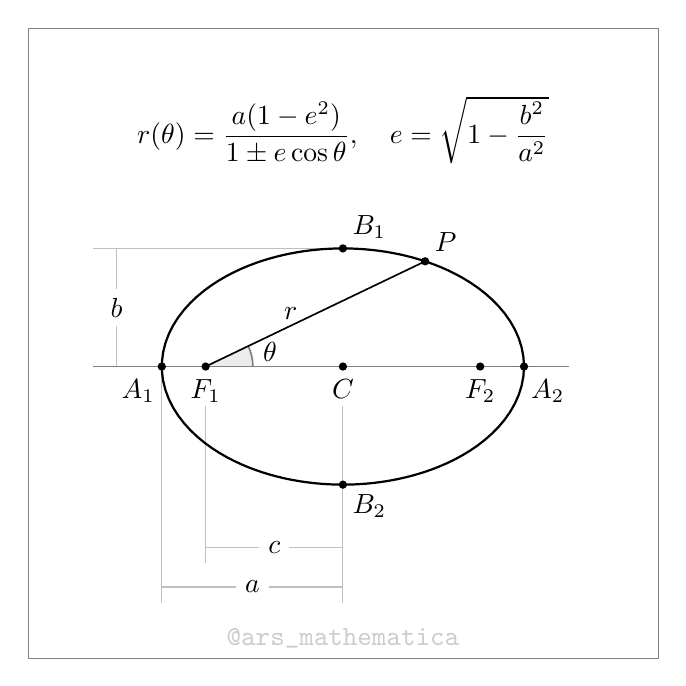
\begin{tikzpicture}

	% márgenes del dibujo
	\draw[help lines] (0,0) rectangle (\L,\L);

	% desplazamiento del origen de coordenadas al centro de la imagen
	\begin{scope}[shift = {(0.5*\L,0.5*\L - 0.3)}]
		
		% definición de las variables
		\tikzmath{
			% parámetros de la elipse
			\a = 2.3; \b = 1.5;
			\c = sqrt((\a)^2 - (\b)^2);
			% ec. de la elipse 
			function f(\x) {
				return \a*\b/sqrt((\a*sin(\x))^2 + (\b*cos(\x))^2);
			};
		};
		
		% expresión
		\node at (0,3) {
			$r(\theta) =
			\dfrac{a(1-e^2)}{1\pm e\cos\theta},
			\quad
			e = \sqrt{1-\dfrac{b^2}{a^2}}$
		};
		
		% def. de las coordenadas importantes
		\coordinate (C) at (0,0);
		\coordinate (F1) at (-\c,0);
		\coordinate (F2) at (+\c,0);
		\coordinate (A1) at (-\a,0);
		\coordinate (A2) at (+\a,0);
		\coordinate (B1) at (0,+\b);
		\coordinate (B2) at (0,-\b);
		
		% elección de un punto arbitrario sobre la elipse
		\tikzmath{ \th = 52; }
		\coordinate (P) at (\th:{f(\th)});
		
		% ángulo
		\pic[
			draw, semithick, gray, fill = gray!15,
			"$\theta$" {black},
			angle radius = 6mm,
			angle eccentricity = 1.4,
		] {angle = F2--F1--P};
		
		% eje horizontal
		\draw[gray] (-1.25*\a - 0.3,0) -- (1.25*\a,0);
		
		% radio vector
		\draw[semithick] (F1) --node[left = 1mm] {$r$} (P);
		
		% elipse
		\draw[thick]
			plot[domain = 0:360, samples = 120]
			(\x:{f(\x)});
		
		% puntos
		\foreach \p in {A1,A2,B1,B2,F1,F2,C,P}
			\fill (\p) circle (1.5pt);
		
		% etiquetas
		\node[above right] at (P) {$P$};	
			
		\node[anchor = base, shift = {(0,-4mm)}] at (C) {$C$};
		
		\node[anchor = base, shift = {(-3mm,-4mm)}] at (A1) {$A_1$};
		\node[anchor = base, shift = {(+3mm,-4mm)}] at (A2) {$A_2$};
					
		\node[anchor = base, shift = {(0,-4mm)}] at (F1) {$F_1$};
		\node[anchor = base, shift = {(0,-4mm)}] at (F2) {$F_2$};
		
		\node[above right] at (B1) {$B_1$};
		\node[below right] at (B2) {$B_2$};
		
		% otras anotaciones			
		{[on background layer]

		\draw[gray!50] (A1) -- ++(0,-3);
		
		\draw[gray!50, shorten <= 5mm] (C) -- (0,-3);	
		\draw[gray!50, shorten <= 5mm] (F1) -- ++(0,-2.5);
		
		\draw[gray!50]
			([yshift = -2.8cm]A1)
				--node[black, fill = white] {$a$}
			([yshift = -2.8cm]C);
			
		\draw[gray!50]
			([yshift = -2.3cm]F1)
				--node[black, fill = white] {$c$}
			([yshift = -2.3cm]C);
		
		\draw[gray!50]
			(B1) -- ++(-1.25*\a - 0.3,0)
			(-1.25*\a,0) --node[black, fill = white] {$b$} ++(0,\b);	
		}
		
	\end{scope}

	% marca de agua
	\node[above, opacity = 0.2]
		at (0.5*\L,0) {\verb|@ars_mathematica|};

\end{tikzpicture}

	
\end{document}